% TEMPLATE for Usenix papers, specifically to meet requirements of
%  USENIX '05
% originally a template for producing IEEE-format articles using LaTeX.
%   written by Matthew Ward, CS Department, Worcester Polytechnic Institute.
% adapted by David Beazley for his excellent SWIG paper in Proceedings,
%   Tcl 96
% turned into a smartass generic template by De Clarke, with thanks to
%   both the above pioneers
% use at your own risk.  Complaints to /dev/null.
% make it two column with no page numbering, default is 10 point

% Munged by Fred Douglis <douglis@research.att.com> 10/97 to separate
% the .sty file from the LaTeX source template, so that people can
% more easily include the .sty file into an existing document.  Also
% changed to more closely follow the style guidelines as represented
% by the Word sample file. 

% Note that since 2010, USENIX does not require endnotes. If you want
% foot of page notes, don't include the endnotes package in the 
% usepackage command, below.

% This version uses the latex2e styles, not the very ancient 2.09 stuff.
\documentclass[letterpaper,twocolumn,10pt]{article}
\usepackage{usenix,epsfig,endnotes}
\usepackage{amsthm}
\usepackage{xcolor}
\usepackage{algorithm}
\usepackage[noend]{algpseudocode}
\usepackage{subfigure}
\usepackage{listings}
\usepackage[hyphens]{url}
\usepackage{xspace}

\newcommand{\annie}[1]{\emph{\color{red}(#1)}}


\begin{document}

%don't want date printed
\date{}

%make title bold and 14 pt font (Latex default is non-bold, 16 pt)
\title{\Large \bf Nation-State Routing}

%for single author (just remove % characters)
%\author{
%{\rm Anne Edmundson}\\
%Princeton University
%\and
%{\rm Roya Ensafi}\\
%Princeton University
%\and
%{\rm Jennifer Rexford}\\
%Princeton University
%\and
%{\rm Nick Feamster}\\
%Princeton University
% copy the following lines to add more authors
% \and
% {\rm Name}\\
%Name Institution
%} % end author

\maketitle

% Use the following at camera-ready time to suppress page numbers.
% Comment it out when you first submit the paper for review.
\thispagestyle{empty}

\subsection*{Abstract}

\section{Introduction}
\label{intro}

There are no restrictions on which national jurisdictions BGP paths must or must not cross.  There is also no way for an Internet user to know or decide which countries her Internet traffic is transitting.  Internet routing is usually studied at the AS (Autonomous System) level - not the nation-state level.  An AS typically controls traffic as it transits it's internal network and then defines policies for filtering, monitoring, and routing traffic to the next AS.  It is becoming increasingly common for governments to require certain actions of ASes, such as enabling wiretapping or performing censorship.  Once Internet traffic enters a country, it is subject to that country's requirements, and subsequently the corresponding ASes' actions.  More and more countries are either trying or have already passed laws that allow for mass surveillance on their citizens~\cite{france_surveillance, netherlands_surveillance, kazak_surveillance}.  Recently, the Investigatory Powers Bill (IP Bill) in the UK, if passed, will require ISPs to store citizens' browsing history for a year, and allow intelligence agencies to collect bulk data on their citizens~\cite{uk_bill}.

Currently, governments are becoming more suspicious about where their citizens' traffic is going, and are facing the challenge of controlling which countries transit the traffic.  Governments and users have been motivated more than ever since the Snowden revelations to avoid countries known for surveillance practices, specifically the United States~\cite{russia_secure_internet, routing_errors, dte}.  More recently, the Safe Harbour agreement, an agreement that allows the free flow of data between the US and the EU, was struck down because it would give the NSA access to EU citizens' personal data~\cite{safe_harbour_illegal, safe_harbour_undecided}.

In response to the Snowden revelations, Brazil has taken great measures to avoid Internet traffic from being wiretapped by the NSA~\cite{brazil_history, brazil_break_from_US, brazil_conference, brazil_conference2, brazil_human_rights}.  Some of the actions that have been taken to avoid NSA surveillance include: building a 3,500 mile long fiber-optic cable from Fortaleza to Portugal (with no use of American vendors), pressing companies such as Google, Facebook, and Twitter (among others) to store data locally, switching its dominant email system (Microsoft Outlook) to a state-developed system called Expresso~\cite{brazil_cable, brazil_us_companies}.  In other efforts, Brazil has been building Internet eXchange Points, which help grow Internet connectivity and performance~\cite{brazil_IXP1, brazil_IXP2}; it also allows them to increase their connectivity with many other countries.  Brazil now has the largest national ecosystem of public Internet eXchange points in the world~\cite{brazil_ixp_ecosystem}.  It has also been shown that over the past few years, the number of ASes in Brazil that are connected internationally have grown significantly~\cite{brazil_international_ases}.  The case of Brazil shows that countries, governments, and Internet users are motivated to avoid surveillance conducted by other countries.

Determining which countries transit Internet traffic, which countries host the only server for a given domain, and which countries are avoidable for a given domain are challenging problems.  The first challeng arises from determining the country-level path that traffic takes; paths can be collected from either the data-plane - IP-level paths - or the control-plane - AS-level paths.  Our work uses the data-plane to analyze traffic paths; in order to determine which countries are on the path, the IP-level path must be mapped to a country-level path.  This is challenging because there is no ground truth for geolocation data; there is no guarantee of accuracy or completeness.  To address this challenge, we use different geolocation tools to increase our confidence in the country-level paths we collect.  More challenges arise in determining how to avoid countries; websites are complex and can fetch data from multiple third parties, which are likely located in different geographic locations, and therefore cross different countries' borders.  The increased usage of anycast IP complicates country avoidance because it gives clients less information about the location of the server from which they are accessing content.  

In this paper, we first shed light on how much traffic is currently transiting countries known for surveillance, with a focus on the US.  Despite the measures taken by different countries to avoid the US, we still see Internet traffic that transits the US.  We conduct a measurement study that helps quantify the existing possibilities for state-sponsored surveillance.  We take Brazil as a case study, and analyze the country-level paths from machines in Brazil to the Brazil Alexa Top 100 domains.  Knowing that Brazil has taken actions to avoid traffic transitting the US, we measure how much traffic is solely transitting the US, and how much traffic is destined for the US.  These are two distinct scenarios.  If the US is solely a country on the path (and not the end point), then there is the possibility for avoiding the US.  If the domain is solely hosted in the US, and therefore destined for the US, then the US cannot be avoided for the given domain.  Using RIPE Atlas probes and the Digital Envoy geolocation service, we find that out of 36,833 traffic paths originating in Brazil to the Brazilian Alexa Top 100 domains, 2,699 are solely transitting the US and the US is the destination for 28,196 of them (this does not necessarily mean that the US is the only possible destination, but it is the destination for Brazilian Internet users)~\cite{ripe_atlas, digital_envoy}.  

Next, we present and implement a new system for surveillance circumvention for Internet users, which finally gives the users some control over where their traffic is flowing.  Because popular web companies are opening or expanding their datacenters in Europe, there are more possible paths to get data~\cite{eu_datacenters}.  It is possible that a path from a client in Brazil to a datacenter in Europe does not pass through any country known for surveillance, but may be a longer path than the best path to a datacenter in the US, as shown in Figure~\ref{fig:intro}.  Our system leverages a geographically diverse set of relay machines that act as proxies to access data from servers located in different geographic regions.  A client will first query an oracle for the best relay to use in order to avoid a given country.  Then the oracle will respond with the IP address of the best relay, which the client will then send it's request to.  The relay will fetch the data from the domain's closest server and return the data to the client. \annie{Add a couple highlights of the results/evaluation section when we get there.}

\begin{figure}
\centering
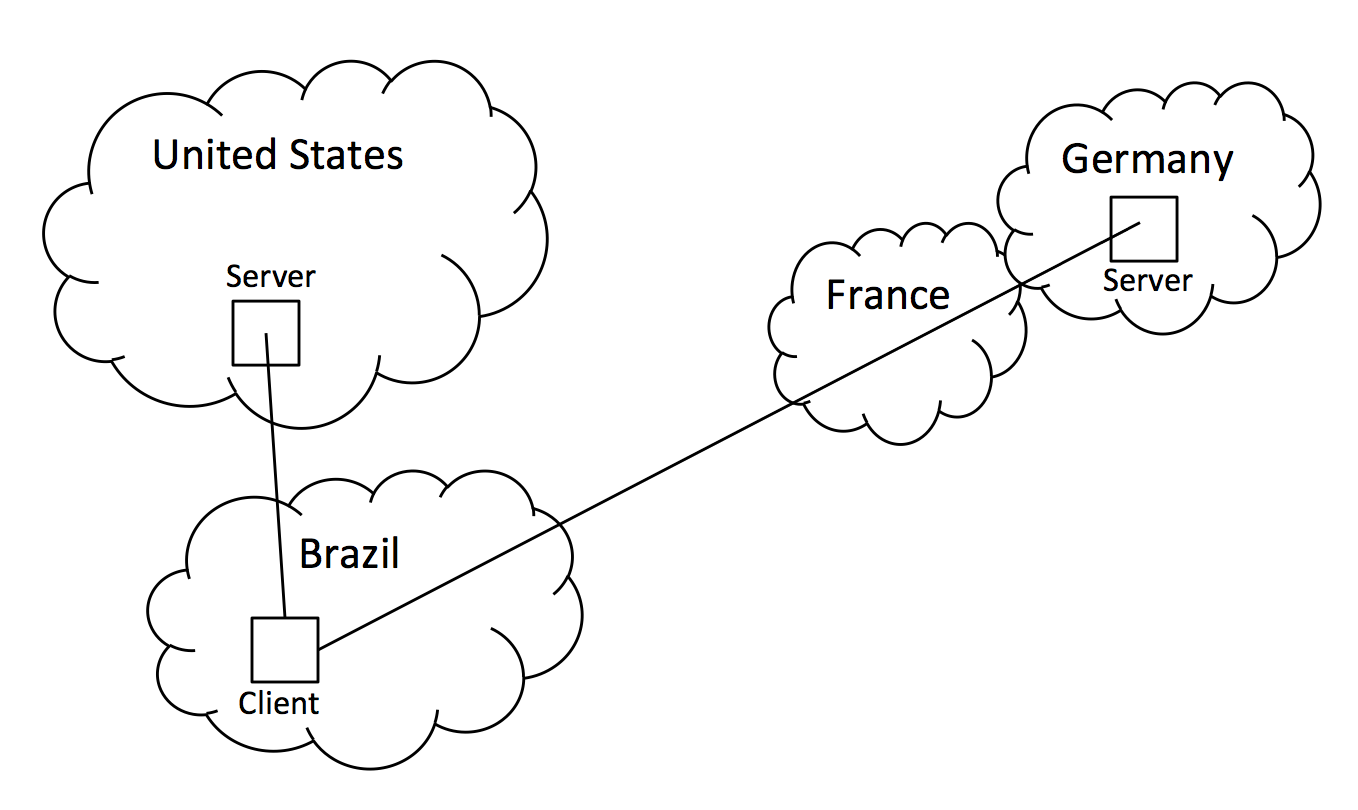
\includegraphics[width=.5\textwidth]{intro_fig}
\caption{A shorter path to a server in a country known for surveillance (U.S.), and a longer path to a georeplicated server in Germany.  The longer path may be more preferred by the client because it doesn't traverse a country with known surveillance practices.}
\label{fig:intro}
\end{figure}

This paper is organized as follows.  In the next section, we describe our research goals, and the challenges in achieving them.  In Section~\ref{datasets} we discuss how and where we collected our data.  We point out the advantages and disadvantages of existing datasets, and justify our decision.  In Section \ref{measure}, we design and execute a measurement study on the country-level paths of Brazil's Internet.  We describe our methodology, as well as results that show which countries Brazil's Internet traffic is traversing.  Next, Section \ref{architecture} introduces SYSTEM, which allows Internet users, ISPs, and Internet services to avoid specified countries, and therefore circumvent surveillance.  Then we explain our implementation of SYSTEM in Section \ref{implementation}.  In Section \ref{evaluation}, we evaluate our system and proposed methods for how well they avoid any given country.  We discuss how our system differs from others and uniquely suits the purpose of country avoidance in Section \ref{discussion}, we review related work in Section \ref{related}, and conclude in Section \ref{conclusion}.

\section{Characterizing Transnational Detours}
\label{datasets}
In this section, we introduce our measurement methods, challenges in conducting the measurements, and our findings on which countries current traffic traverses.

\begin{figure*}[t]
\centering
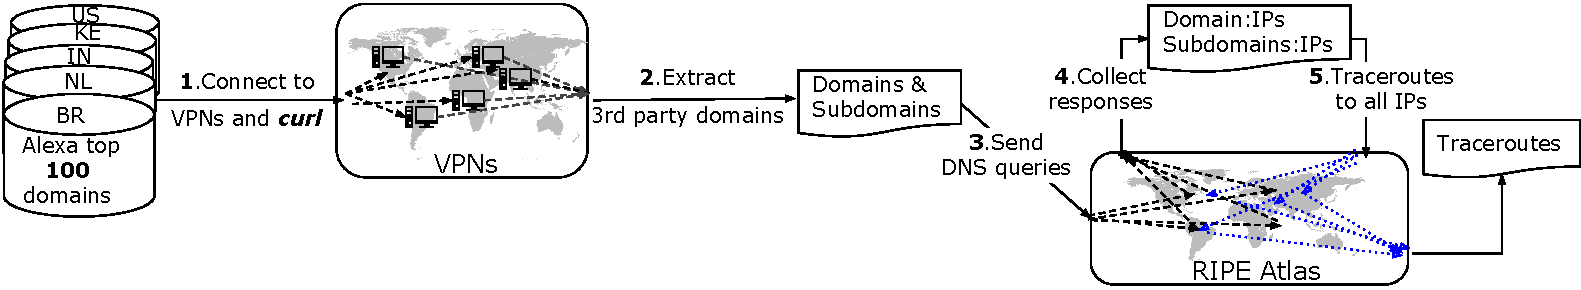
\includegraphics[width=.9\textwidth]{Current-Traffic_fig}
\caption{The measurement pipeline to study current traffic routes.}
\label{fig:pipeline1}
\end{figure*}

\begin{figure}[t]
\centering
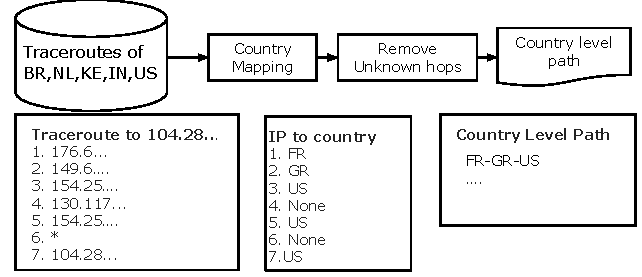
\includegraphics[width=.5\textwidth]{Analysis-Pipeline1}
\caption{The measurement pipeline to analyze traceroutes.}
\label{fig:analysis_pipeline}
\end{figure}

\subsection{Measurement Pipeline}
\label{pipeline}
We use the data plane to measure traffic paths; we analyze the reported hops of traceroute measurements to find which countries are on the path from a client in a particular country to a popular domain.  The reverse path is just as important as the forward path, and often the reverse path is different from the forward path; we measure how symmetric the forward and reverse paths are the country-level in Section \ref{path_sym}, and also explain how the exclusion of the reverse path provides a lower bound on the number of countries that traffic traverses.  Using traceroutes to measure transnational detours is new; prior work used BGP routing tables to \textit{infer} country-level paths~\cite{karlin2009nation}.  Because we conduct active measurements, which are limited by our resources, we make a tradeoff and study five countries, as opposed to all countries' Internet paths.  Figure \ref{fig:pipeline1} shows the steps taken for this measurement; first we identify a set of popular domains, then we use RIPE Atlas probes to query DNS with these domains, and traceroute to the DNS responses.  The measurements were conducted on January 31st, 2016.  Our analysis involves the steps seen in Figure \ref{fig:analysis_pipeline}; we map traceroutes to country-level paths.

\subsubsection{Resource Limitations}
\label{resource_limits}
To our knowledge, the publicly available traceroute datasets suitable for our goal are from iPlane~\cite{madhyastha2006iplane} and CAIDA (Center for Applied Internet Data Analysis)~\cite{caida}.  The iPlane project uses PlanetLab~\cite{planetlab} nodes to run traceroutes to all unique AS-level paths in the BGP routing table.  This project also has historical data as far back as 2006.  Unfortunately, because iPlane uses PlanetLab nodes, which have been shown to mostly use the Global Research and Education Network (GREN), the traceroutes from PlanetLab nodes will not be representative of typical Internet users' traffic paths~\cite{banerjee2004interdomain}.  The other publicly available dataset, from CAIDA, ran traceroutes from different vantage points around the world, but to randomized destination IP addresses that cover all /24s.  This is also not sufficient for what we wanted to measure because a typical Internet user is going to access a domain that will be locally resolved; the user will not input a specific IP address in their browser.  

We chose to run active measurements that would be most representative of an Internet user.  We chose to run DNS and traceroute measurements from RIPE Atlas probes, which are hosted all around the world and in many different settings, including home networks~\cite{ripe_atlas}.  RIPE Atlas probes can use the local DNS resolver, which would give us the best estimate of the traceroute destination.

Despite the options RIPE Atlas provides, there were still restrictions that made measurements challenging.  To conduct any measurement on a RIPE Atlas probe, it costs a certain amount of credits, and we were therefore restricted by the number of credits we had.  Additionally, RIPE Atlas imposes rate limits on the number of concurrent measurements and the number of credits that an individual user can spend per day.  We address these challenges in two ways: 1) we reduce the number of necessary measurements we must run on RIPE Atlas probes by conducting traceroute measurements to a single IP address in each /24 (as opposed to all IP address returned by DNS) because all IP addresses in a /24 belong to the same AS, and should therefore be located in the same geographic area; 2) use a different method---VPN connections---to get a vantage point within a foreign country, which is still representative of an Internet user in that country.

\subsubsection{Path Asymmetry}
\label{path_sym}
Previous work has shown that paths are not symmetric most of the time---the forward path from point A to point B does not match the reverse path from point B to point A~\cite{he2005routing}.  Most work on path asymmetry has been done at the AS level, but not at the country level.  Our measurement methods only take the forward path (from client to domain or relay) into account, and not the path from the domain or relay to the client.  

We conducted a study to measure path asymmetry at the country granularity; if country-level paths are symmetric, then the results of our measurements would be representative of the forward {\it and} reverse paths, but if the country-level paths are asymmetric, then our measurement results only provide a lowerbound on the number of countries that could potentially conduct surveillance.  Using 100 RIPE Atlas probes located around the world, and 8 Amazon EC2 instances, we ran traceroute measurements from every probe to every EC2 instance and from every EC2 instance to every probe.  After geolocating the IPs to countries, we analyzed the paths for symmetry.  First, we compared the set of countries on the forward path to the set of countries on the reverse path; this yielded about 30\% symmetry.  What we wanted to know is whether or not the reverse path has more countries on it than the forward path.  We measured how many reverse paths were a subset of the respective forward path; this was the case for 55\% of the paths.  

The results of this measurement are not convincing enough to state that country-level paths are symmetric, and therefore our measurements and results represent a lowerbound on the number of countries that transit traffic; our results are a lowerbound on how many unfavorable countries transit a client's traffic.

\subsubsection{Traceroute Origination and Destination Selection}
As discussed above, we used RIPE Atlas probes in each of the five countries we studied.  Each of these countries had varying amounts of probes hosted in the country, ranging from about 75 probes to many hundreds.  Because of the resource restrictions, we could not use all probes in each of the countries.  We selected the set of probes that had unique ASes in the country to get the widest representation of origination (starting) points.

For destinations, we used the Alexa Top 100 domains in each of the respective countries, as well as the 3rd party domains that are requested as part of an original web request.  To obtain these 3rd party domains we {\tt curl} (fetch) each of the Top 100 domains, but we must do so from within the country we are studying.  There is no current functionality to {\tt curl} from RIPE Atlas probes, so we establish a VPN connection within each of these countries to {\tt curl} each domain and extract the 3rd party domains; we {\tt curl} from the client's location in case web sites are customizing content based on the region of the client.

\subsubsection{Country Mapping}
\label{c_map}
Geolocation services and tools have been studied and proposed, and continue to be a growing research area.  Because that is not the primary focus of our work, we use MaxMind's geolocation service to map IP addresses to their respective countries~\cite{maxmind}.   Our study requires country-level paths, which is a coarser granularity than either city granularity or latitude-longitude granularity.  Previous work has studied the inaccuracy of geolocation services, but the evaluation was at the latitude-longitude granularity~\cite{huffaker2011geocompare}; we observe less inaccuracy at the country-level.  To address the incompleteness of the data, we cleaned up our IP to country mapping by removing all IP addresses that resulted in a `None' response when querying MaxMind, which causes our results to provide a conservative estimate of the number of countries that traffic passes through. It is important to note that removing `None' responses will \textit{always} produce a conservative estimate, and therefore we are \textit{always} underestimating the amount of potential surveillance.  An example of this can be seen in Figure \ref{fig:analysis_pipeline}.  This method provides a lower bound on the number of countries that are included on the path, and therefore a lower bound on the countries that can conduct surveillance.  

\subsection{Results}

%%%% ADD THIS TO datasets.tex
\newcolumntype{d}[1]{D{.}{.}{#1}}
\newcommand{\headrow}[1]{\multicolumn{1}{c}{\adjustbox{angle=45,lap=\width-0.5em}{#1}}}
\newcolumntype{P}[1]{>{\raggedright\arraybackslash}p{#1}}
\newcommand{\ra}[1]{\renewcommand{\arraystretch}{#1}}
\begin{table}[t]
\centering
\ra{1.2}
\resizebox{\columnwidth}{!}{%
\begin{tabular}{@{}ld{3.2}d{3.2}d{3.2}d{3.2}d{3.2}@{}}
%\multicolumn{1}{l}{}    & \headrow{Host} & \headrow{Transit} & \headrow{Host} & \headrow{Transit} &\headrow{Host} &\headrow{Transit} &\headrow{Host}   &\headrow{Transit} &\headrow{Host}  &\headrow{Transit} \\

\textit{Country}    & \headrow{Brazil}  & \headrow{Netherlands}   & \headrow{India} & \headrow{Kenya} & \headrow{United States}\\
\toprule
Brazil             &.169    &-     &-    & -  & - \\ \midrule
Canada             &.001    &.007     &.015      &.006       & -  \\
United States      &\cellcolor[HTML]{F7BE81}.774    &\cellcolor[HTML]{F7BE81}.454      &\cellcolor[HTML]{F7BE81}.629      &\cellcolor[HTML]{F7BE81}.443        &\cellcolor[HTML]{F7BE81}.969    \\ \midrule
France             &.001    &.022      &.009      &.023       &.001 \\
Germany            &.002    &.013      &.014      &.028       &.001  \\
Great Britain      &-  &.019     &.021     &.032       &.002 \\
Ireland            &.016    &.064      &.027       &.108       &.001   \\
Netherlands        &.013    &\cellcolor[HTML]{F7BE81}.392      &.101      &\cellcolor[HTML]{F7BE81}.200      &.024  \\
Spain              &.001    &-     & -    &  -     &-    \\ \midrule
Kenya              &-        &  -    & -    &.022        &-  \\
Mauritius          &  -      & -    & -   &.004       & -  \\
South Africa       & -       & -     & -  &.021       &-  \\ \midrule
United Arab Emirates & -     & -     & -   &.011        &-  \\
India              &  -      & -     &.053    &.002        &-  \\
Singapore          & -       &.002     &\cellcolor[HTML]{F7BE81}.103      &.027       & - \\\hline
\end{tabular}
}
\caption{Fraction of paths that end in each country in default routes.}
\label{tab:host}
\end{table}

\begin{table}[t]
\centering
\ra{1.2}
\resizebox{\columnwidth}{!}{%
\begin{tabular}{@{}ld{3.2}d{3.2}d{3.2}d{3.2}d{3.2}@{}}
%\multicolumn{1}{l}{}    & \headrow{Host} & \headrow{Transit} & \headrow{Host} & \headrow{Transit} &\headrow{Host} &\headrow{Transit} &\headrow{Host}   &\headrow{Transit} &\headrow{Host}  &\headrow{Transit} \\

\textit{Country}    & \headrow{Brazil}  & \headrow{Netherlands}   & \headrow{India} & \headrow{Kenya} & \headrow{United States}\\ \toprule
Brazil              &1.00       & -   & -     & -     & -\\ \midrule
Canada                &.013       &.007     &.016       &.008      &.081 \\
United States        &\cellcolor[HTML]{F7BE81}.844        &\cellcolor[HTML]{F7BE81}.583     &\cellcolor[HTML]{F7BE81}.715      &\cellcolor[HTML]{F7BE81}.616       &\cellcolor[HTML]{F7BE81}1.00 \\ \midrule
France                 &.059     &.102      &.104       &.221      &.104 \\
Germany                 &.005       &.050    &.032      &.048      &.008 \\
Great Britain                &.024       &\cellcolor[HTML]{F7BE81}.140     &\cellcolor[HTML]{F7BE81}.204      &\cellcolor[HTML]{F7BE81}.500      &.006 \\
Ireland                &.028       &.106      &.031     &.133      &.006 \\
Netherlands                 &.019        &1.00      &.121      &\cellcolor[HTML]{F7BE81}.253      &.031 \\\hline
Spain                  &.176       &.004     & -     & -      &- \\ \midrule
Kenya                 & -       &-    & -      &1.00      &- \\\hline
Mauritius                  & -       & -     & -      &\cellcolor[HTML]{F7BE81}.322       &- \\
South Africa                 &-        & -    & -     &\cellcolor[HTML]{F7BE81}.334       &- \\ \midrule
United Arab Emirates                  &.00003        & -    & -     &.152       &- \\
India               &  -    &.0007    &1.00     &.058     &.0005 \\
Singapore                 &.0009        &.002     &\cellcolor[HTML]{F7BE81}.270       &.040       &.003 \\ \midrule
\end{tabular}
}
\caption{Fraction of paths that each country transits in default routes.}
\label{tab:transit}
\end{table}

Table \ref{tab:host} shows the five studied countries along the top of the table, and the countries that host their traffic along the Y axis.  For example, the United States is the endpoint of 84\% of the paths that originate in Brazil.  A ``-'' represents the case where no traffic ended in that country.  For example, no Brazilian paths ended in South Africa. Table \ref{tab:transit} shows the fraction of paths that transit certain countries (along the Y axis).

\begin{finding}[Hosting Diversity]
About half of the top domains in each of the five countries studied are hosted in a single country.
\end{finding}
First we analyzed hosting diversity; this shows us how many unique countries in which a domain is hosted---the more countries that a domain is hosted in creates a greater chance that the content is replicated in a favorable country, and could potentially allow a client to circumvent an unfavorable country.  We queried DNS from 26 vantage points around the world, which are shown in Figure \ref{fig:world}; we chose this set of locations because they are geographically diverse.  Figure~\ref{fig:host_diversity} shows two common hosting cases: 1) CDNs, and 2) a single hosting country.  This shows that many domains are hosted in a single unique country, which leads us to our next analysis---where are these domains hosted, and which countries are traversed on the way to reach these locations.

\begin{figure}[t]
\centering
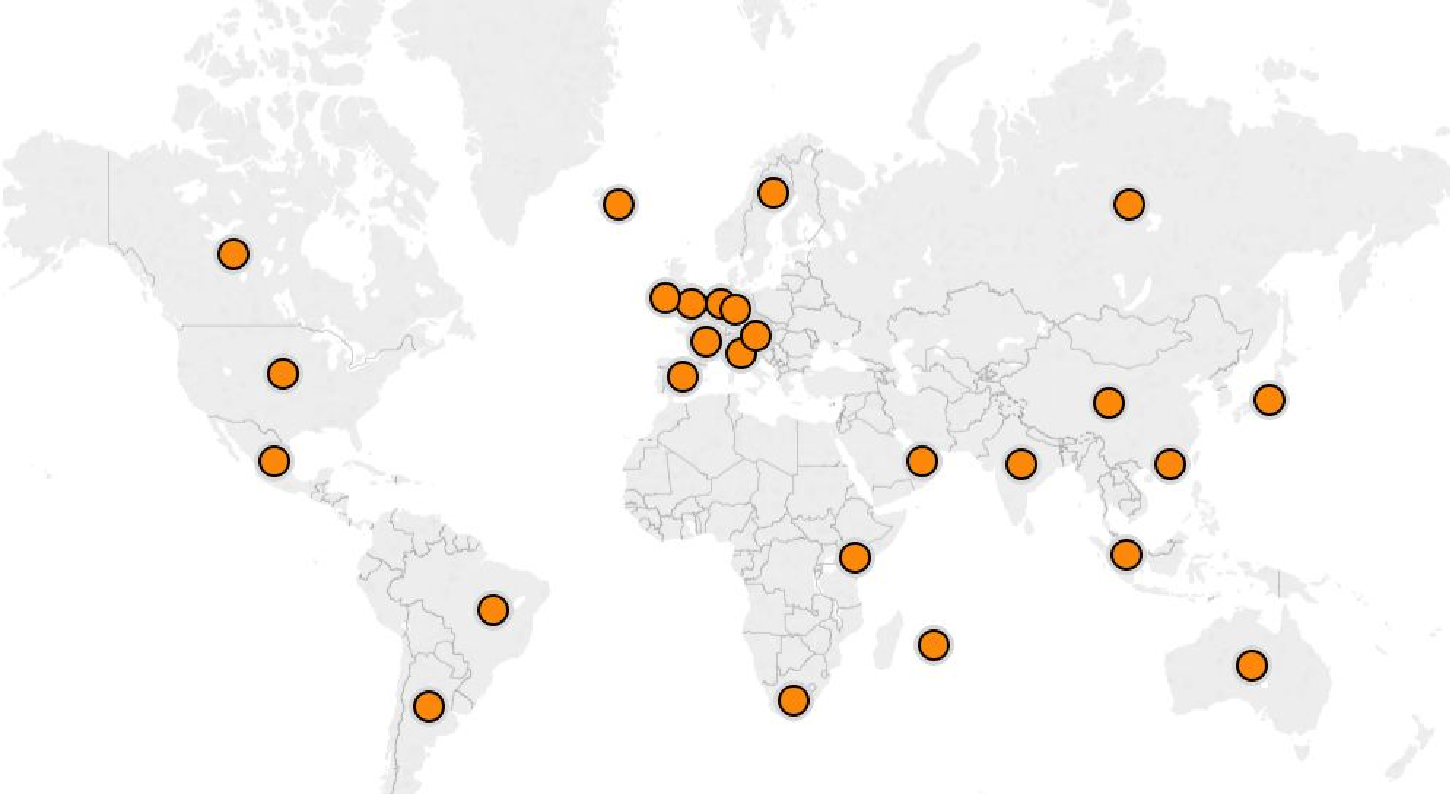
\includegraphics[width=\columnwidth]{World-DNS}
\caption{The locations of vantage points in measuring hosting diversity.}
\label{fig:world}
\end{figure}

\begin{figure}[t]
\centering
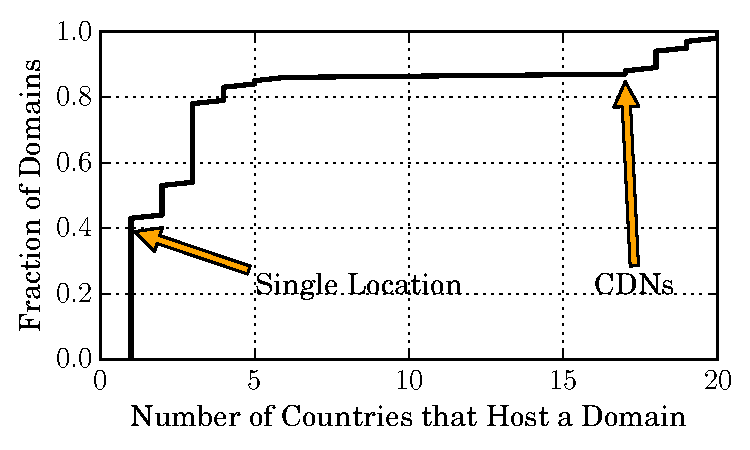
\includegraphics[width=\columnwidth]{domain_hist_US1}
\caption{The number of Alexa Top 100 US Domains hosted in different countries.}
\label{fig:host_diversity}
\end{figure}

\begin{finding}[Domain Hosting]
The most common destination among all five countries studied is the United States: 77\%, 45\%, 63\%, 44\%, and 97\% of paths originating in Brazil, Netherlands, India, Kenya and the United States, respectively, are currently reaching content located in the United States.
\end{finding}
The fraction of paths that are hosted in various countries can be seen in Table~\ref{tab:host}.  Despite the amount of country-level hosting diversity, we see the majority of paths from all five countries ending in a single country: the United States.  This is significant because the United States is a known surveillance state, and therefore these percentages represent the amount of foreign traffic that the United States can conduct surveillance on.  Our results also show the Netherlands is a common hosting location for traffic originating in the Netherlands, India, and Kenya.

%For Indian traffic, in addition to the 63\% hosted in the United States and the 10\% hosted in the Netherlands, another 10\% is hosted in Singapore.  Hosting in these countries can best be explained by the number of underwater cables with landing points in both India and Singapore~\cite{cablemap}.  More specifically, there is a cable that directly connects Chennai, India and Changi North, Singapore, and is owned by Tata Communications, which is one of the top global Internet providers (in terms of transitted IP space)~\cite{bakers}.  

%For Kenyan traffic, the United States hosts 44\% of the content, but Ireland hosts 10\%; Ireland is a popular hosting location for U.S. companies due to its relaxed enforcement of privacy in the private sector \annie{I got this information from Joel Reidenberg - how do I cite that?  I'll also look to see if I can find any publications that discuss this}.  

\begin{finding}[Domestic Traffic]
All of the countries studied (except for the United States) host content for a small percentage of their own traffic; they also host a small percentage of the their respective country code top-level domains.
\end{finding}
For traffic that originates in Brazil, only 17\% of it also ends in Brazil.  Only 5\% and 2\% of Indian and Kenyan traffic, respectively, end in the originating country. 
For Kenya, 24 of the Top 100 Domains are .ke domains, and of these 24 domains only 5 are hosted within Kenya.  29 out of 40 .nl domains are hosted in the Netherlands; 4 of 13 .in domains are hosted in India; 18 of 39 .br domains are hosted in Brazil.  Interestingly, all .gov domains were hosted in their respective country. 

\begin{finding}[Transit Traffic]
Surveillance states (specifically the United States and Great Britain) transit the largest portion of traffic in comparison to any other (foreign) country.
\end{finding}
Brazilian traffic traverses the United States on 84\% of the paths; therefore, the United States can conduct surveillance on 84\% of the traffic originating in Brazil, despite Brazil's strong efforts in avoiding United States surveillance.  Even though India and Kenya are geographically distant, 72\% and 62\% of their traffic transits the United States.   

Great Britain and the Netherlands are on the path for a significant percentage of traffic originating in India and Kenya.  50\% and 20\% of paths that originate in Kenya and India transit Great Britain.  Traffic that traverses the Netherlands can be explained by the large IXP located there; traffic that traverses Great Britain is likely due to being on the path between the originating country and the final destination in a European country.

Mauritius, South Africa, and the United Arab Emirates transit 32\%, 33\%, and 15\% of traffic from Kenya.  There are direct underwater cables from Kenya to Mauritius, and from Mauritius to South Africa~\cite{cablemap}.  Additionally, there is a cable from Mombasa, Kenya to Fujairah, United Arab Emirates.  This accounts for the large percentages of traffic that pass through these countries.

\begin{finding}[Tromboning Traffic]
Brazilian and Netherlands traffic often trombones to the United States, despite the prevalence of IXPs in both countries.
\end{finding}
As mentioned above, the percentage of domestic traffic in some of the countries studied is extremely small.  For India, only 5\% of traffic is domestic and for Kenya, 2\% is domestic; despite the small amount of domestic traffic, some of this traffic trombones.  This can be seen better in the cases of Brazil and the Netherlands; 
Figures \ref{fig:trombone_netherlands}, \ref{fig:trombone_brazil}, and \ref{fig:trombone_kenya} show the amount of paths that trombone to different countries for the Netherlands, Brazil, and Kenya. 24\% of all paths originating in the Netherlands (62\% of domestic traffic) trombone to a foreign country before returning to the Netherlands. Despite Brazil's strong efforts in building IXPs to keep local traffic local, we can see that their traffic still trombones to the United States.  This is due to IXPs being seen as a threat by competing commercial providers; providers are sometimes concerned that ``interconnection'' will result in making business cheaper for competitors and stealing of customers~\cite{ixp_policy}.  It is likely that Brazilian providers see other Brazilian providers as competitors and therefore as a threat at IXPs, which causes them to peer with international providers instead of other local providers.

\begin{figure*}[t!]
\begin{minipage}{\linewidth}
\begin{subfigure}[b]{.32\linewidth}
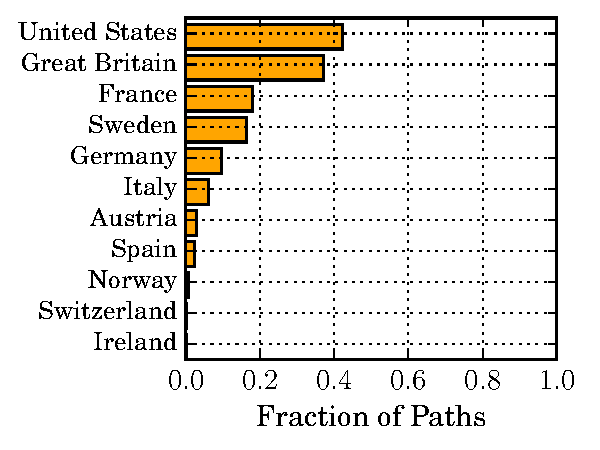
\includegraphics[width=\linewidth]{nl_trombone_new11}
\caption{The Netherlands.\label{fig:trombone_netherlands}}
\end{subfigure}\qquad
\begin{subfigure}[b]{.32\linewidth}
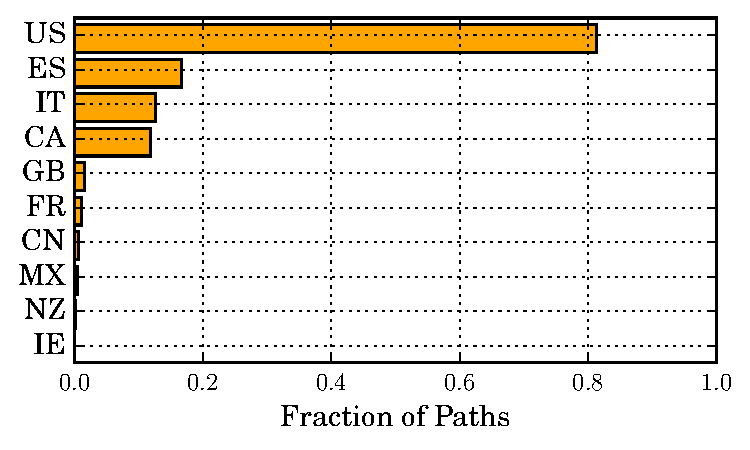
\includegraphics[width=\linewidth]{br_trombone_new11}
\caption{Brazil.\label{fig:trombone_brazil}}
\end{subfigure}\qquad
\begin{subfigure}[b]{.32\linewidth}
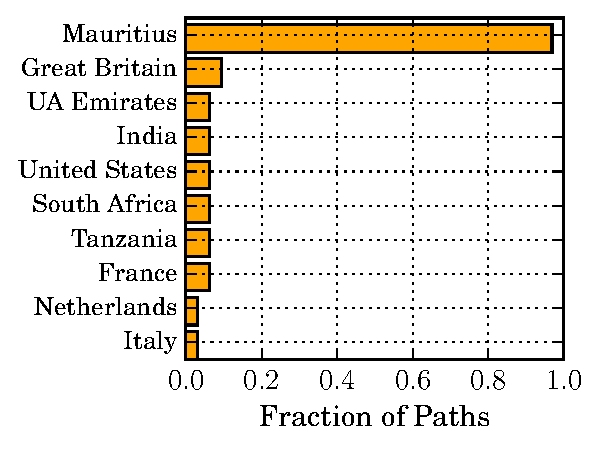
\includegraphics[width=\linewidth]{ke_trombone_new11}
\caption{Kenya.\label{fig:trombone_kenya}}
\end{subfigure}
\end{minipage}
\caption{The countries that tromboning traffic from the Netherlands, Brazil, and Kenya transits.}
\label{fig:trombone}
\end{figure*}

  %Traffic that should be kept local is susceptible to surveillance because it transits two well-known surveillance states.  

\begin{finding}[United States as an Outlier]
The United States hosts 97\% of the content that is accessed from within the country, and only 6 foreign countries---France, Germany, Ireland, Great Britain, and the Netherlands---- host content for the other 3\% of traffic.
\end{finding}
Most of the results discussed thus far have shown that Brazilian, Netherlands, Indian, and Kenyan traffic often transit surveillance states, most notably the United States.  The results from studying traffic that originates in the United States are drastically different from those of the other four countries.  The other four countries hosted very small amounts of their own traffic, whereas the United States hosts 97\% of the content that is accessed from within the country.  Only 13 unique countries are ever on a path from the United States to a domain in the top 100 (or third party domain), whereas 30, 30, 25, and 38 unique countries are seen on the paths originating in Brazil, Netherlands, India, and Kenya.  

%There are only 6 foreign countries---France, Germany, Ireland, Great Britain, and the Netherlands----that host content for traffic originating in the United States, and the fraction of content hosted in these countries is less than 4\% combined.

\subsection{Limitations}
The measurement methods that we described in Section~\ref{datasets} are not without limitations.  First, our study is solely based on IPv4 routes, which likely differ from IPv6 routes.  Here we also discuss limitations with IPv4, country mapping accuracy, and traceroute completeness.

\subsubsection{IPv4}
The measurements we conducted only collect and analyze IPv4 paths, and therefore all IPv6 paths are left out of our study.  IPv6 paths likely differ from IPv4 paths as not all routers that support IPv4 also support IPv6.  Future work includes studying IPv6 paths and which countries they transit, as well as a comparison of country avoidability between IPv4 and IPv6 paths. 

\subsubsection{Country Mapping}
Previous work has shown that there are fundamental challenges in deducing a geographic location from an IP address, despite using different methods such as DNS names of the target, network delay measurements, and host-to-location mapping in conjunction with BGP prefix information~\cite{padmanabhan2001investigation}.  While it has been shown that there are inaccuracies and incompleteness in MaxMind's data~\cite{huffaker2011geocompare}, the focus of this work is on measuring and avoiding surveillance, and not on geolocation algorithms, we therefore used a pre-existing geolocation service. Additionally, we discuss how we address inaccuracies and incompleteness in Section \ref{c_map}.

\subsubsection{Traceroute Accuracy and Completeness}
Our study is limited by the accuracy and completeness of traceroute.  Anomalies can occur in traceroute-based measurements~\cite{augustin2006avoiding}, but most traceroute anomalies do not cause an overestimation in surveillance states.  The incompleteness of traceroutes, where a router does not respond, causes our results to underestimate the number of surveillance states, and therefore also provides a lower bound on surveillance.

\section{Nation-State Routing: Default \\Routes}
\label{measure}

\newcommand{\headrow}[1]{\multicolumn{1}{c}{\adjustbox{angle=45,lap=\width-0.5em}{#1}}}
\newcolumntype{P}[1]{>{\raggedright\arraybackslash}p{#1}}
\begin{table*}[t]
\centering
\begin{tabular}{|P{37mm}|cc|cc|cc|cc|cc|}
\multicolumn{1}{l}{}    & \headrow{Host} & \headrow{Transit} & \headrow{Host} & \headrow{Transit} &\headrow{Host} &\headrow{Transit} &\headrow{Host}   &\headrow{Transit} &\headrow{Host}  &\headrow{Transit} \\\hline
\textit{Country}    &\multicolumn{2}{c|}{\textit{Brazil}}   &\multicolumn{2}{c|}{\textit{Netherlands}}   &\multicolumn{2}{c|}{\textit{India}} &\multicolumn{2}{c|}{\textit{Kenya}} &\multicolumn{2}{c|}{\textit{United States}}\\
\hline\hline
Brazil             &.169     &1.00   &     &  &   &   &    &     &  & \\\hline
Canada             &.001     &.013   &.007     &.007  &.015    &.016   &.006    &.008     &  &.081 \\\hline
France             &.001     &.059   &.022     &.102  &.009    &.104   &.023    &.221     &.0013  &.104 \\\hline
Germany             &.002     &.005   &.013     &.050  &.014    &.032   &.028    &.048     &.0013  &.008 \\\hline
Great Britain             &.00006     &.024   &.019     &.140  &.021    &.204   &.032    &.500     &.0024  &.006 \\\hline
India             &    &   &     &.0007  &.053   &1.0   &.002    &.058     &  &.0005 \\\hline
Ireland             &.016     &.028   &.064     &.106  &.027    &.031   &.108    &.133     &.0012  &.006 \\\hline
Kenya             &    &   &     &  &   &   &.022    &1.0     &  & \\\hline
Mauritius             &     &   &     &  &    &   &.004    &.322     &  & \\\hline
Netherlands             &.013     &.019   &.392     &1.0  &.101    &.121   &.200    &.253     &.024  &.031 \\\hline
Singapore             &    &.0009   &.002     &.002  &.103    &.270   &.027    &.040     &  &.003 \\\hline
South Africa             &    &   &     &  &   &   &.021    &.334     &  & \\\hline
Spain             &.001     &.176   &    &.004  &   &   &   &     &  & \\\hline
United Arab Emirates             &     &.00003   &     &  &   &   &.011    &.152     &  & \\\hline
United States             &.774     &.844   &.454     &.583  &.629    &.715   &.443    &.616     &.969  &1.0 \\\hline
\end{tabular}
\caption{Fraction of paths that each country sees in default routes.}
\label{tab:transit_host}
\end{table*}

As Internet traffic crosses international borders, it becomes subject to the wiretapping policies of the national jurisdiction in which it is transitting.  We study five different countries, Brazil, Netherlands, India, Kenya, and the United States, and measure which countries are transitting their traffic.  The methods we use are described in Section \ref{pipeline1}, and in this section we discuss our findings.

\subsection{Hosting Diversity}
First we look at hosting diversity.  This shows us how many unique countries in which a domain is hosted -- the more countries that a domain is hosted in creates a greater chance that the content is replicated in a favorable country, and could potentially allow a client to circumvent an unfavorable country.  By querying DNS from 26 vantage points around the world, we found that there is hosting diversity among the Alexa Top 100 Domains.  About half of the Alexa Top 100 Domains in each of the five countries studied are hosted in more than one country.  This can be seen in Figure~\ref{fig:host_diversity}.  The amount of hosting diversity motivates the potential for circumventing surveillance states.  We next look at which countries are currently transitting and hosting Internet traffic, and measure whether traffic is going to replicas in surveillance states (when they may not need to).

\begin{figure}
\centering
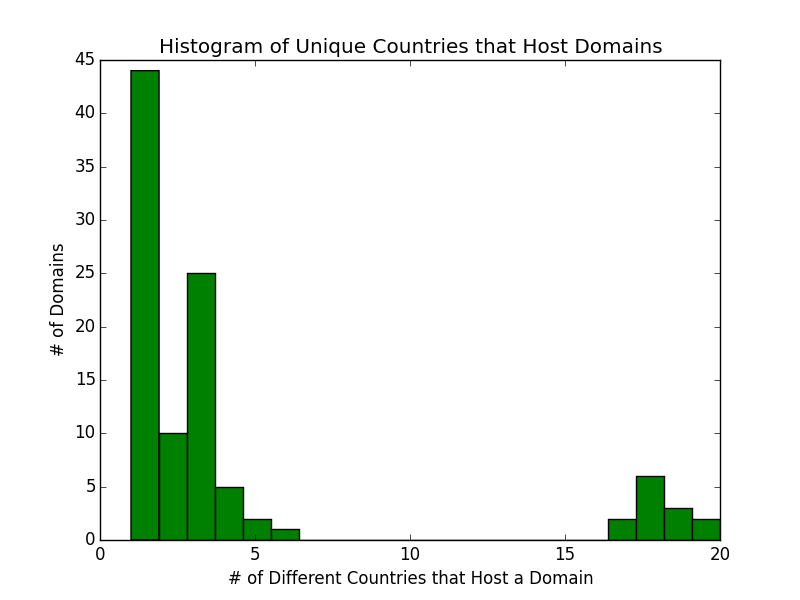
\includegraphics[width=.5\textwidth]{host_domains_hist_US}
\caption{The number of Alexa Top 100 US Domains hosted in different countries.}
\label{fig:host_diversity}
\end{figure}

\subsection{Trend 1: Surveillance States Host Domains}
\label{trend1}
Despite the amount of country-level hosting diversity, we see the majority of paths from all five countries ending in a single country.  The fraction of paths that are hosted in various countries can be seen in Table~\ref{tab:transit_host}.  The most common destination among all five countries studied is the United States: 77\%, 45\%, 63\%, 44\%, and 97\% of paths originating in Brazil, Netherlands, India, Kenya and the United States, respectively, are currently reaching content located in the United States.  This is significant because the United States is a known surveillance state, and therefore these percentages represent just a portion of foreign traffic that the United States can conduct surveillance on.  Our results also show the Netherlands as a common hosting location for traffic originating in the Netherlands, India, and Kenya.

For Indian traffic, in addition to the 63\% hosted in the United States and the 10\% hosted in the Netherlands, another 10\% is hosted in Singapore.  This can best be explained by the number of underwater cables with landing points in both India and Singapore~\cite{cablemap}.  More specifically, there is a cable that directly connects Chennai, India and Changi North, Singapore, and is owned by Tata Communications, which is one of the top global Internet providers (in terms of transitted IP space)~\cite{bakers}.  

For Kenyan traffic, the United States hosts 44\% of the content, but Ireland hosts 10\%; Ireland is a popular hosting location for U.S. companies due to it's relaxed enforcement of privacy in the private sector.  

It is also worth noting that most of the countries studied host a small percentage of their own traffic.  For traffic that originates in Brazil, only 17\% of it also ends in Brazil.  Only 5\% and 2\% of Indian and Kenyan traffic, respectively, end in the originating country.  In addition, only a fraction of country code top-level domains are hosted with in the respective country.  For Kenya, 24 of the Top 100 Domains are .ke domains, and of these 24 domains only 5 are hosted within Kenya.  29 out of 40 .nl domains are hosted in the Netherlands; 4 of 13 .in domains are hosted in India; 18 of 39 .br domains are hosted in Brazil.  Interestingly, all .gov domains were hosted in their respective country.

\subsection{Trend 2: Traffic Transits Surveillance States}
Similar to the trend of hosting domains, the United States also transits a large portion of foreign traffic -- it transits a larger portion of traffic than it hosts.  Brazilian traffic traverse the United States on 84\% of the paths; therefore, the United States can conduct surveillance on 84\% of the traffic originating in Brazil, despite Brazil's strong efforts in avoiding United States surveillance.  Even though India and Kenya are geographically distant, 72\% and 62\% of their traffic transits the United States.  Of the five countries studied, the Netherlands has the lowest percentage of traffic that transits the United States at 58\%.  

Great Britain and the Netherlands are on the path for a significant percentage of traffic originating in India and Kenya.  50\% and 20\% of paths that originate in Kenya and India transit Great Britain.  Traffic that traverses the Netherlands can be explained by the large IXP located there; traffic that traverses Great Britain is likely due to being on the path between the originating country and the final destination in a European country.

Mauritius, South Africa, and the United Arab Emirates transit 32\%, 33\%, and 15\% of traffic from Kenya.  There are direct underwater cables from Kenya to Mauritius, and from Mauritius to South Africa.  Additionally, there is a cable from Mombasa, Kenya to Fujairah, United Arab Emirates.  This accounts for the large percentages of traffic that pass through these countries.

\subsection{Trend 3: Tromboning Traffic Transits Surveillance States}

As mentioned in Section \ref{trend1}, the percentage of domestic traffic in some of the countries studied is extremely small.  For India, only 5\% of traffic is domestic and for Kenya, 2\% is domestic; despite the small amount of domestic traffic, some of this traffic trombones.  This can be seen better in the cases of Brazil and the Netherlands; figure \ref{trombone_netherlands} shows the amount of paths that trombone to differing countries for the Netherlands.

\begin{figure}
\centering
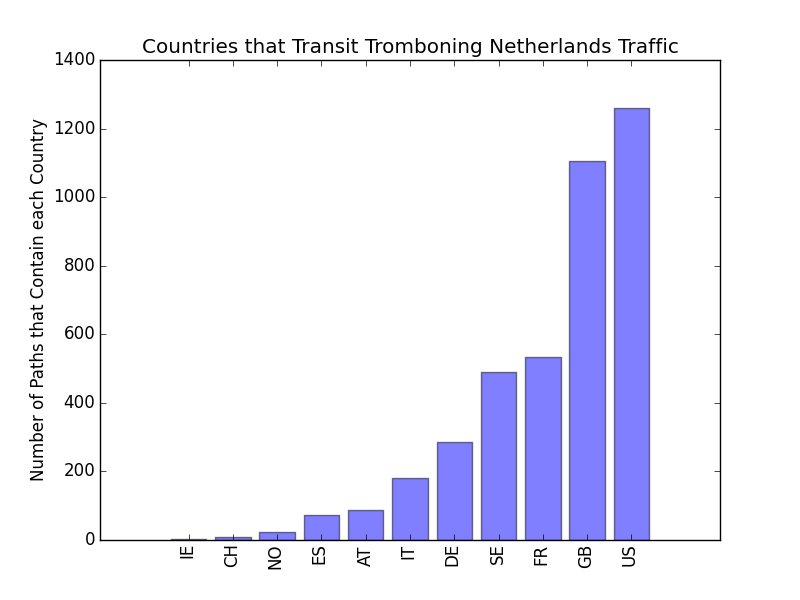
\includegraphics[width=.5\textwidth]{nl_trombone_no_none2}
\caption{The countries that tromboning Netherlands traffic transits.}
\label{fig:trombone_netherlands}
\end{figure}

24\% of all paths originating in the Netherlands (62\% of domestic traffic) trombone to a foreign country before returning to the Netherlands; The most common countries traffic trombones to are the United States and Great Britain.  Traffic that should be kept local is susceptible to surveillance because it transits two well-known surveillance states.  For Brazil, 5\% of all traffic starts in the Netherlands, transits a foreign country, and returns to the Netherlands (30\% of domestic traffic trombones).  The most common country traffic trombones to is the United States. 

\subsection{United States as an Outlier}

Most of the results discussed thus far have shown that Brazilian, Netherlands, Indian, and Kenyan traffic often transit surveillance states, most notable the United States.  The results from studying traffic that originates in the United States are drastically different from those of the other four countries.  The other four countries hosted very small amounts of their own traffic, whereas the United States hosts 97\% of the content that is accessed from witin the country.  Only 13 unique countries are ever on a path from the United States to a domain in the Top 100 (or third party domain), whereas 30, 30, 25, and 38 unique countries are seen on the paths originating in Brazil, Netherlands, India, and Kenya.  There are only 6 foreign countries that host content for traffic originating in the United States, and the fraction of content hosted in these countries is less than 4\% combined.

\section{System Architecture}
\label{architecture}

In this section, we discuss \system{}, a system for avoiding a specified country when accessing a webpage.

\subsection{Threat Model}
\label{threat}
This system is targeting an attacker who is at the nation-state level, and practices wiretapping on Internet traffic within the nation-state.  This type of attacker can appear on either the forward or reverse path, as shown in Figure~\ref{fig:attacker}. An attacker can also conduct surveillance on parts of webpages by being on the path from the client to some source that is requested by an initial page load; for example, a client accesses foo.com, and foo.com uses a Javascript file from bar.com, but bar.com is located in a different location.  An attacker can see the traffic between the client and bar.com, but not the client and foo.com.  This is depicted in Figure~\ref{fig:domains_attacker}.

\begin{figure}[t]
\begin{minipage}[c][11cm][t]{.5\textwidth}
  \centering
  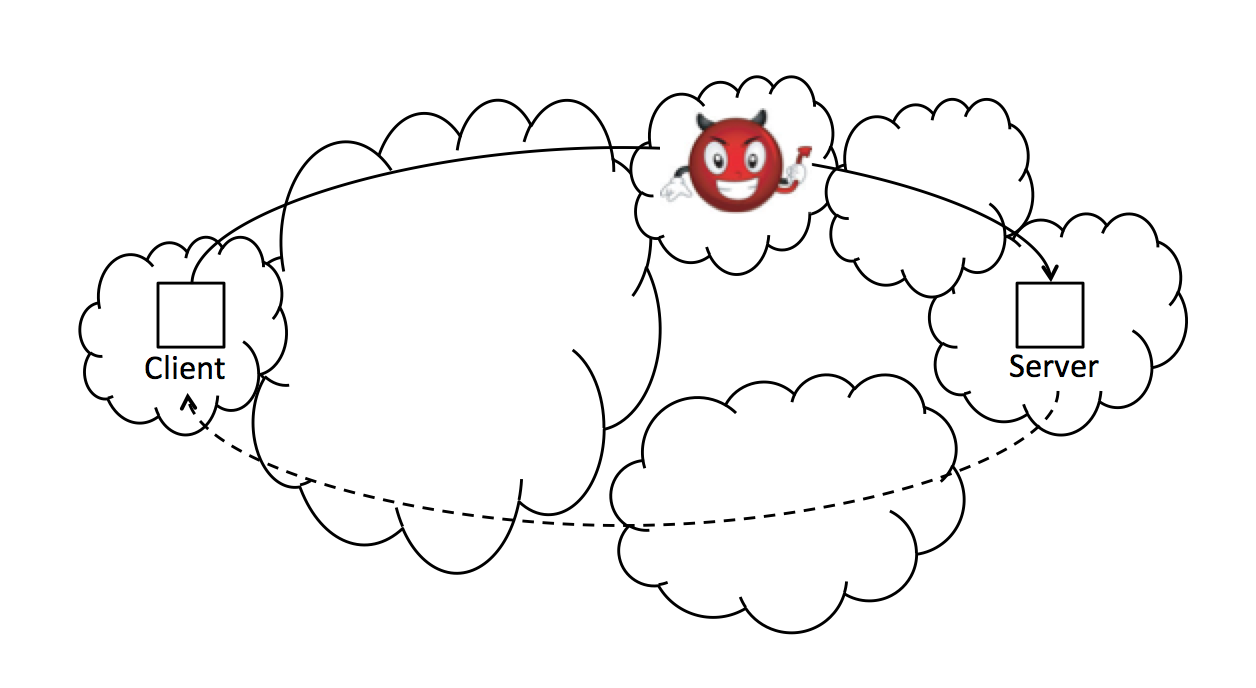
\includegraphics[width=.99\textwidth]{forward_evil}
  \subcaption{An attacker on the forward path.}
  \label{fig:forward_attack}\par\vfill
  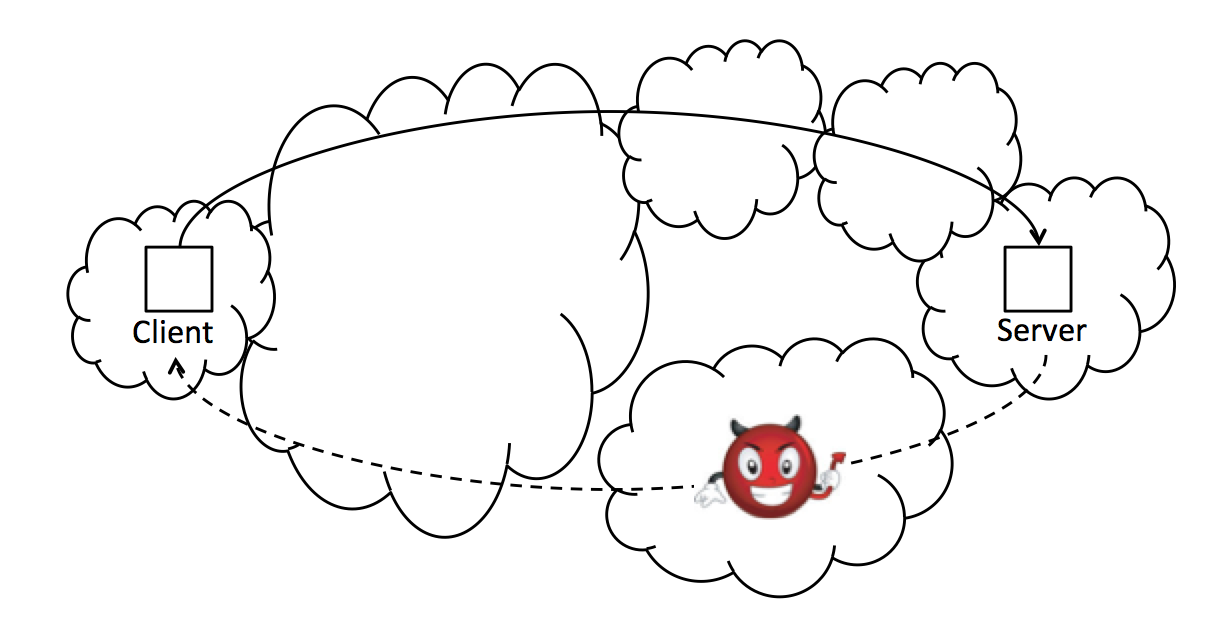
\includegraphics[width=.99\textwidth]{reverse_evil}
  \subcaption{An attacker on the reverse path.}
  \label{fig:reverse_attack}
\end{minipage}
\caption{An attacker can be on the forward or reverse path.}
\label{fig:attacker}
\end{figure}

\begin{figure}[t]
\centering
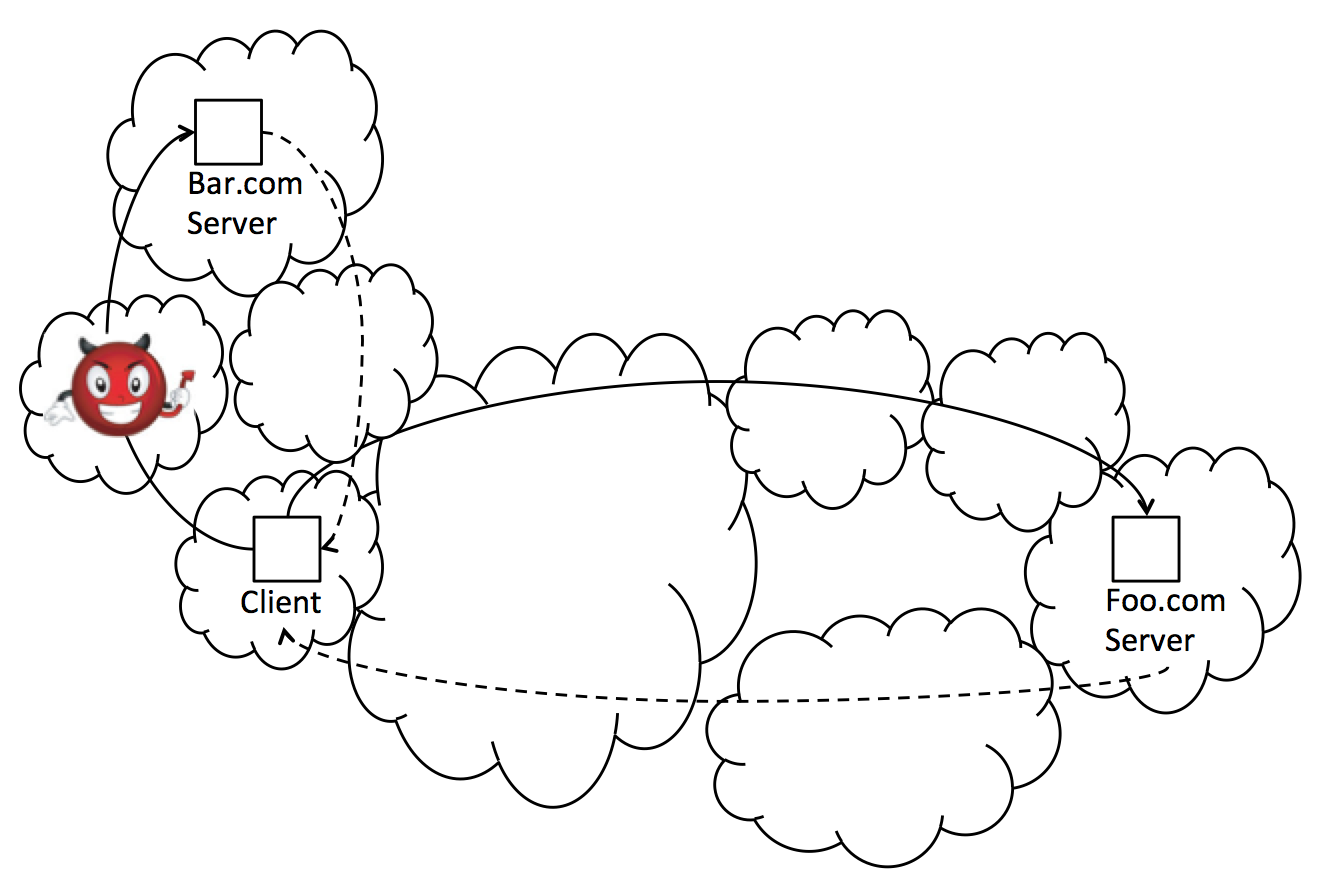
\includegraphics[width=.5\textwidth]{subsequent_request_attacker}
\caption{An example attacker on the path from the client to a third party domain's server (bar.com), which was fetched due to an initial request for foo.com.}
\label{fig:domains_attacker}
\end{figure}

\subsection{Design Goals}

With the attacker described in Section~\ref{threat} in mind, \system{} has three goals: singular country avoidance, avoiding colluding countries, and usability.  

\paragraph{Country Avoidance.}  The system should allow an Internet user, a client, to access web content without having her traffic travel through a country that she specifies, particularly countries that conduct surveillance.  The specified country should be avoided on both the forward and reverse paths, as they have been shown to be asymmetric, and thus a country may be on the reverse path, but not on the forward path~\cite{he2005routing}.  

\paragraph{Colluding Countries Avoidance.}  There have been agreements between countries to share surveillance data; this is analagous to colluding adversaries~\cite{fiveeyes}.  This system will allow clients to specify multiple countries to avoid, and the system will attempt to avoid all specified countries.  For the purposes of simplicity, the examples and descriptions in this paper will include only one country to avoid, but the system will be designed to handle multiple colluding countries.

\paragraph{Usability.} In order for the system to be used, it must be usable from both the client- and server-side.  All participants in the system must be required to do as little work as possible to use the system.  We envision the system growing, and our goals for the long-term would also be scalability and performance.

We assume that relays, clients, servers, and oracles are not malicious, and that no other attacks, such as Man-in-the-Middle, BGP prefix hijack, etc., are occuring.

\subsection{Architecture Overview}

Figure~\ref{fig:overview} shows the steps that occur when a client visits www.foo.com, using a standard browser. Both the oracle and the server maintain country-level path information, which is described in more detail in Section~\ref{maps}.

\begin{enumerate}
\item A client queries the oracle by supplying a domain and a country to avoid.  
\item The oracle searchs for a suitable relay, such that the specified country is not on the client to relay path, the relay to server path, and the relay to client path.  Once this relay is found, it responds to the client with the IP address of the relay.
\item The client sends the web request to the relay.
\item The relay forwards the request to the closest server that contains the domain.
\item The server determines if the server to relay path avoids the given country.  If so, then it sends the response to the relay. If not, then it will check if any of the geo-replicated servers have a path to the relay that does not include the given country; if there is such a path, then it uses it, otherwise, country avoidance is not possible for this request.
\item The relay forwards the response to the client.
\end{enumerate}

\begin{figure}[t]
\centering
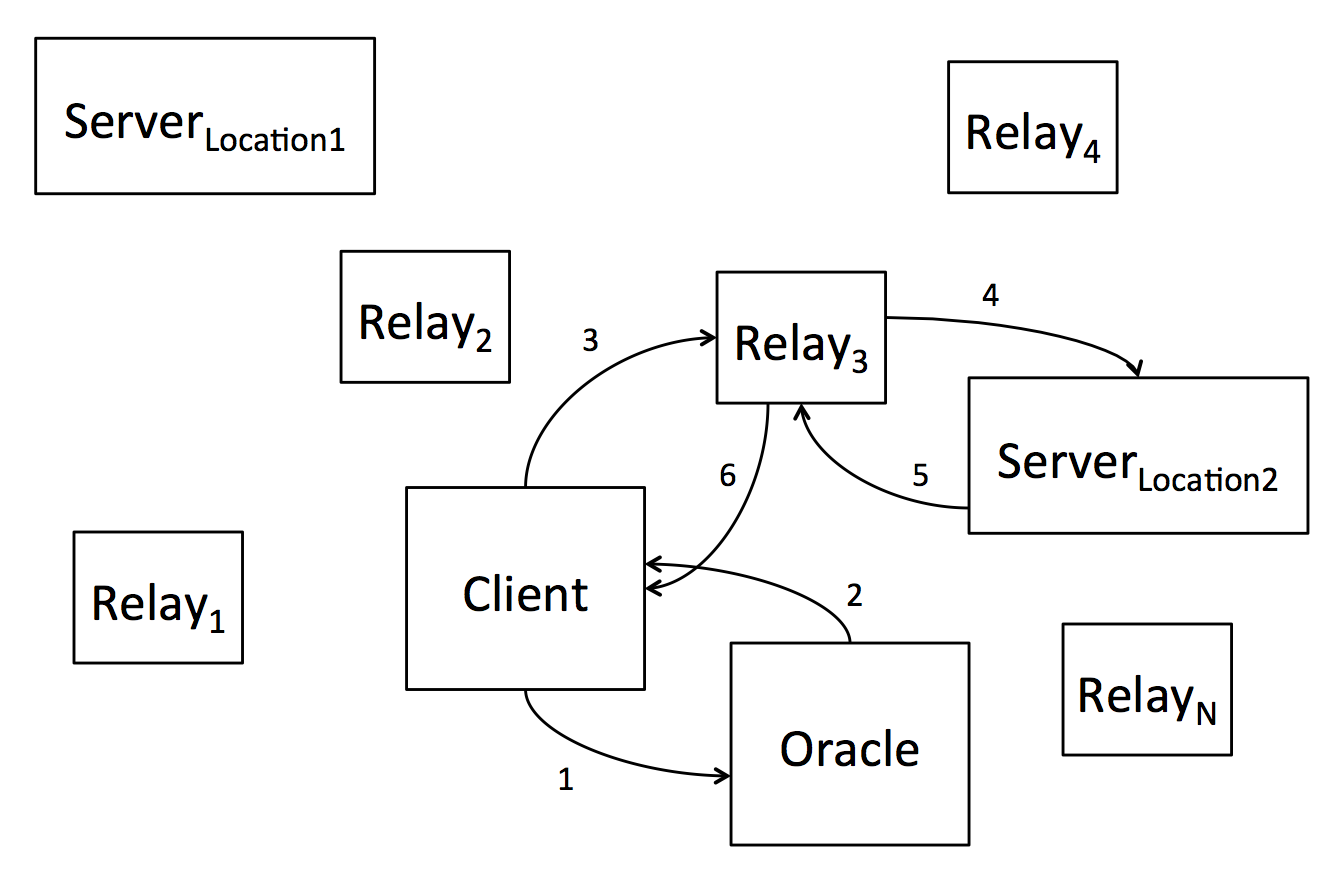
\includegraphics[width=.5\textwidth]{system_overview}
\caption{Using \system{}, the steps involved in requesting web content.}
\label{fig:overview}
\end{figure}

Based on this system design, we can see that there are more possible paths that an attacker can be on.  Figure~\ref{fig:advanced_threat} shows the possible places that a specified country (to be avoided) may be; these include the path from the client to the relay, the relay to the server, the server to the relay, and the relay to the client.  This increased attack space is because forward and reverse paths are asymmetric; research has shown that forward and reverse paths are asymmetric at the AS-level, but to our knowledge, no work has looked at the asymmetry of country-level paths~\cite{he2005routing}.  We found that the forward and reverse paths are asymmetric at the country level; we used RIPE Atlas probes to run traceroute measurements between pairs of probes.  Then we mapped the IP-level path to the country-level path.  Some country-level paths were symmetric, but we found others that were asymmetric; for example, a path from Brazil to Germany (189.112.0.1 to 185.13.208.1) has the country-level path Brazil $\rightarrow$ Venezuela $\rightarrow$ United States $\rightarrow$ Germany, whereas a path from Germany to Brazil (185.13.208.1 to 189.112.0.1) has the path Germany $\rightarrow$ Great Britain $\rightarrow$ United States $\rightarrow$ Brazil.  This shows that we cannot assume symmetric country-level paths. This is compounded by the secondary requests that are issued when the page is loaded on the client's browser.  

\begin{figure}[t]
\centering
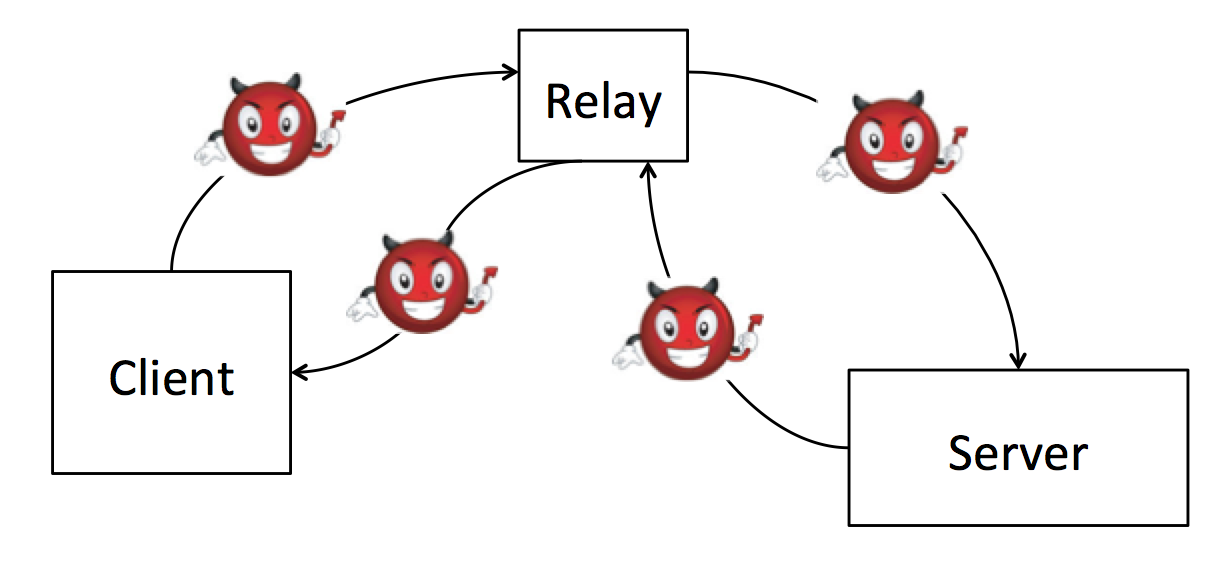
\includegraphics[width=.5\textwidth]{all_attackers}
\caption{The possible locations a country (to be avoided) may reside when using \system{}.}
\label{fig:advanced_threat}
\end{figure}

\subsubsection{Client} The client queries the oracle for a suitable relay and then uses that relay to access web content.  First, the client checks it's cache for the domain; if it is in the cache, then the client uses the relay IP address that is in associated with the domain in the cache.  It's important to note that the client's cache is refreshed twice as often as the oracle refreshes it's paths.  If the domain is not in the cache, then the client sends a query containing the domain and the country to avoid to the oracle.  The client will then recieve a response that is the IP address of a suitable relay for avoiding the specified country.  This (domain, relay IP address) pair will be added to the client's cache and the web request for the domain will be sent to the relay IP address.  Then the client waits for a response from the relay to display in the client's browser.  This process is repeated for each source that is requested during the web page load.  

\subsubsection{Oracle} The oracle contains information about the country-level path for the following source-destination pairs:

\begin{itemize}
\item Client to Relay
\item Relay to Server
\item Relay to Client
\end{itemize}

It contains these mappings for every client, every relay, and every popular server/CDN.  Once it receives a query from a client, it searchs the mappings for a relay such that the country to avoid is not on the client to relay path, relay to server path, and relay to client path.  Once a relay is found that satisfies these requirements, it sends the IP address of the relay to the client.  More information on the initialization, freshness, and maintenance of the mappings is discussed in Section~\ref{maps}.

\subsubsection{Relay} The relays act as proxies for clients so that it appears that a client is in a different geographic location; this allows the client to access the same web content on a different georeplicated server.  The proxy accepts requests from clients, locally resolves the domain, and forwards the request to the closest replicated server.  It then waits for a response from the server, and forwards it to the client.   

\subsubsection{Server} The server contains information about the country-level path for the server to relay path.  Once the server receives a web request, it checks it's mappings and if the country to avoid is not on the path from server to relay, then it sends the response to the relay.  If the country to avoid is on the path from server to relay, then it can check if any of it's georeplicated servers have a path to the relay that avoid the specified country.  If there is some server location that can avoid the specified country, then the response is sent from that server \annie{check the Internet Cache Protocol detail to see if this is feasible}.  Otherwise, the country is unavoidable, and response is sent through the specified country.

\subsection{Mapping Creation and Maintenance}
\label{maps}

Both the oracle and the servers must generate and maintain mappings of pairs of machines to the country-level paths.  The oracle must maintain the country-level paths from: all clients to all relays, all relays to all popular servers/CDNs, all relays to all clients.  The server must maintain the country-level paths from all of the georeplicated servers (for the domain) to all relays.  

The mappings for the oracle are initialized by using RIPE Atlas probes to conduct traceroute measurements from client subnets to all relays.  Traceroute measurements are also run from all relays to all popular servers/CDNs and to all client subnets.  Once these IP-level paths are calculated, the oracle uses a geolocation tool to map the IP-level paths to country-level paths.  These are then stored in the oracle as:

\begin{itemize}
\item (client,relay) $\rightarrow$ country-level path
\item (relay,server) $\rightarrow$ country-level path
\item (relay,client) $\rightarrow$ country-level path
\end{itemize}

The same method is used on the server-side to generate the (server,relay) $\rightarrow$ country-level path mapping.  These mappings are recalculated once per day because it has been shown that BGP paths change that often~\cite{} \annie{find citation for this}.

\section{Evaluation}
Using the \system{} implementation, we evaluate the system on it's ability to avoid a given country, performance, and scalability in terms of storage and costs.

\subsection{Country Avoidance}
As the primary goal of the system is to provide country avoidance for a given 
country, we measured how much avoidance the system achieves.  We did so by first 
calculating the number of {\it default} paths that avoid a given country.  Then 
we added a single relay, and calculated how many domains the client could 
access without traversing through the given country.  This was repeated for 
the remaining two relays.  The evaluation was conducted under the condition that 
the client wished to avoid different countries when accessing the Netherlands top 
100 domains, and the results are shown in Figure \ref{fig:avoidance_eval}.  Each 
line represents the fraction of domains accessible while avoiding the country that 
the line represents.  For example, 46\% of domains are accessible without traversing 
the United States when \system{} is not being used (0 relays), and if \system{} is 
used, then 63\% of domains are accessible with traversing the United States.

\begin{figure}[b!]
\centering
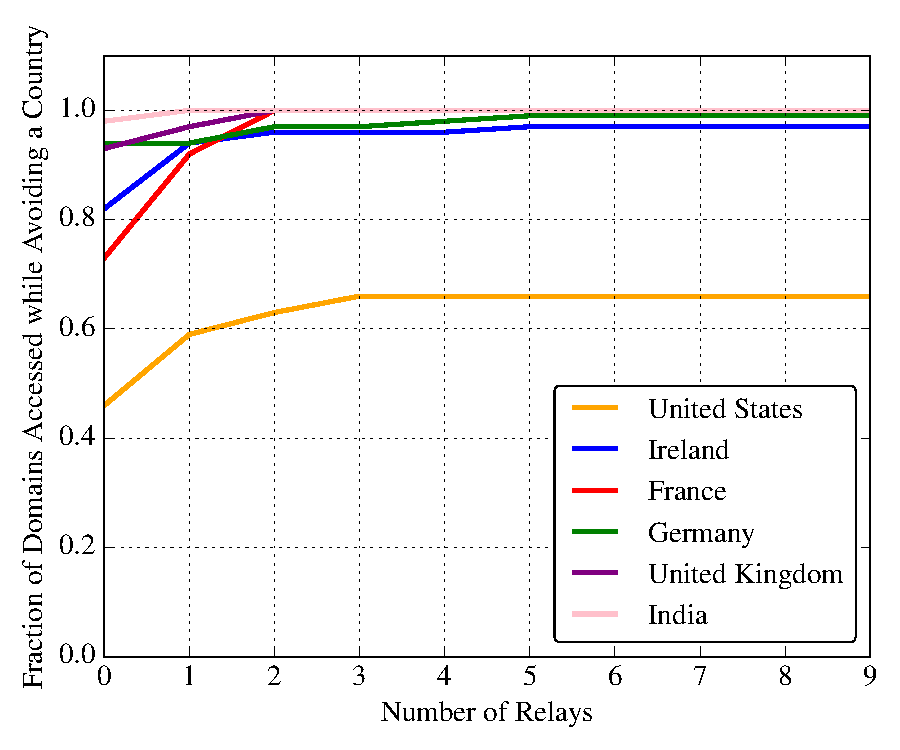
\includegraphics[width=.5\textwidth]{avoidance_n_relays}
\caption{How much avoidance different numbers and locations of relays achieve.}
\label{fig:avoidance_eval}
\end{figure}

It is evident that \system{} helps a client avoid a foreign country, as the 
fraction of domains accessible without traversing 
the specified country without \system{} is lower than with \system{}.  Additionally, 
it is clear that adding the first relay provides the greatest increase in 
provided avoidance, while subsequent relays provide a significantly 
smaller amount (or no) additional avoidance.

Figure \ref{fig:avoidance_eval} also clearly shows how much more difficult (or 
impossible) it is to avoid the United States than it is to avoid any other 
country.  Only 63\% of domains can be accessed while avoiding the United States, 
whereas almost all domains can be accessed while avoiding any other given 
country.  This confirms the results presented in Section \ref{avoid_results}, and 
emphasizes how crucial the systematization of the measurements is for enabling 
\system{}.

\subsection{Performance}
A system is not usable if the performance is significantly worse than what a user
is accustomed to.  To measure the performance of \system{}, we measure both 
the throughput and latency.

To measure throughput, we ran {\tt wget} for each 
of the top 100 domains from the client machine in the Netherlands, while 
using the PAC file.  Based on the {\tt wget} output, we calculate the number 
of seconds to access content using our system. Figure \ref{fig:latency} shows 
the CDF of the ratio of direct throughput to \system{} throughput. 

\begin{figure}[t]
\centering
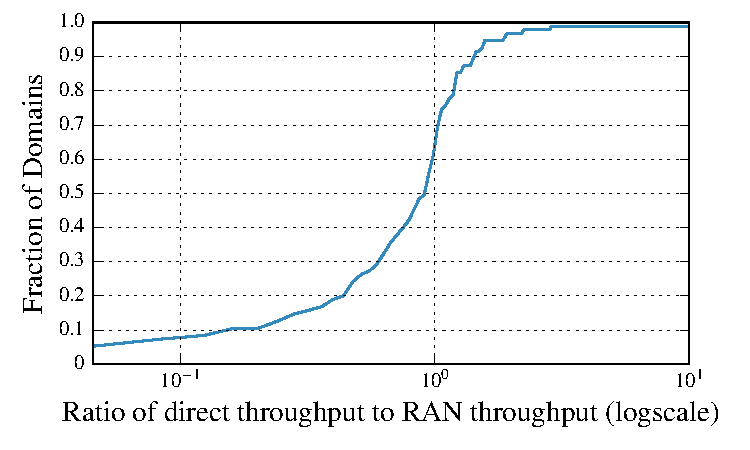
\includegraphics[width=.5\textwidth]{throughput}
\caption{Latency difference when accessing a webpage via \system{} vs. default paths. 
The difference is calculated by \system{} latency minus default latency, and represents 
the additional latency cost of our system.}
\label{fig:latency}
\end{figure}

We can see that the throughput of \system{} is not significantly worse than that 
of default paths.  In fact, in some cases the performance of \system{} is {\it 
better} than that of default paths.  This could be a result of the relays 
keeping local traffic local, or due to a closer content replica being selected. 
These results show that \system{}'s performance is comparable to the performance 
of accessing domains without \system{}.

To measure the latency of \system{}, we ran a {\tt curl} command to each of the 
top 100 domains from the client machine in the Netherlands, while using the PAC file. 
This provided the time to first byte (TTFB); we found the TTFB for both \system{} and 
direct paths, and the results are shown in Figure \ref{fig:latency}.  

\begin{figure}[t]
\centering
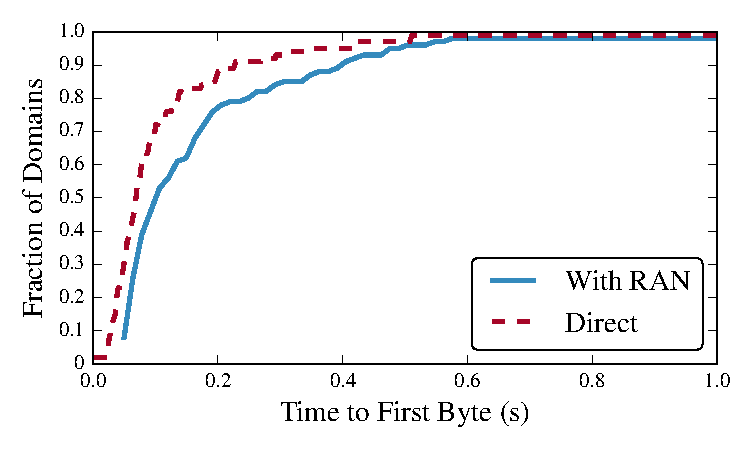
\includegraphics[width=.5\textwidth]{latency}
\caption{Latency difference when accessing a webpage via \system{} vs. default paths. 
The difference is calculated by \system{} latency minus default latency, and represents 
the additional latency cost of our system.}
\label{fig:latency}
\end{figure}

The median TTFB for direct paths is .0685, and for \system{} paths, it is .10075.  Additionally, 
the 90th percentile for direct and \system{} paths is .2253 and .40352, respectively.  This 
shows that the system's latency is greater by a factor of 2 (or 20-40ms).  \annie{Say if this is 
significant or not, especially as it relates to page load times.}

\subsection{Storage}
As the number of clients increase, and subsequently the number of paths being 
computed increases, the amount of storage must remain reasonable.  The storage 
used by paths can be calculated:

\[Storage(D,R,C) = (D x R) + 2(C x R) + (C x D) \]

D is the number of domains; R is the number of relays; C is representative of the number of 
clients.  While C {\it represents} clients, it is not the number of clients using the 
system --- it is the number of vantage points the system uses to measure paths 
from client locations.  For the prototype with a single client, the storage space for all 
paths computed is 480KB.  As there is a single PAC file for all clients in 
a country, C will grow much slower than if there was a different PAC file for 
each individual client.  There are 196 countries in the world today, and if 
paths and a PAC file were generated for each country, with 100 domains, and 
three relays, the storage would only be 94MB.  This provides plenty of storage 
for increasing the number of domains included in the PAC file or increasing 
the number of relays in the system.

\subsection{Costs}
In addition to storage, the cost of the measurements used in the system must 
be taken into account.  RIPE Atlas credits are a limited resource, and therefore 
we must earn more credits than we are spending on measurements.  The cost 
in credits follows the equation:

\[Credit\_Cost(D,R,C) = COST_{traceroute}((C x R) + (C x D))\]

Currently, the $COST_{traceroute}$ is 60, resulting in a prototype cost of 6,180 
credits, but because these paths are updated each hour, then 
the daily credit cost is 148,320 credits.  In return for hosting a RIPE Atlas 
probe, we earn 216,000 credits per day, which will support our existing 
prototype.  In order to provide for more clients, more domains, or more 
resources, we can tune the system to re-compute paths less frequently (only when necessary).

\section{Discussion}

\subsection{Why existing tools don't work}

\subsection{Alibi Routing}

\subsection{Security - Other Attackers}

\section{Related Work}
\label{related}

\paragraph{Nation-state routing analysis.}  Shah and
Papadopoulos recently measured international routing detours---paths that originate
in
one country, cross international borders, and then return to the
original country)---using public Border Gateway Protocol~(BGP) routing tables~\cite
{shah2015characterizing}. 
The study discovered 2 million detours each month out
of 7 billion total paths); the study also characterized the detours based
on detour dynamics and persistence.  Our work differs because it {\em actively}
measures traceroutes, yielding a more precise measurement of the path traffic is
likely to take, as opposed to analyzing BGP
routes.  Obar and Clement analyzed traceroutes
that started and ended in Canada, but tromboned through the United
States, and argued that
this is a violation of Canadian network
sovereignty~\cite{obar2012internet}. 
Karlin \ea developed a framework for country-level
routing analysis to study how much influence each country has over
interdomain routing~\cite{karlin2009nation}.  This work measures the
centrality of a country using BGP routes and AS-path inference; in contrast, our work uses active 
measurements and measures avoidability of a given country. 

\paragraph{Mapping national Internet topologies.}  Roberts \ea developed a method
for mapping national networks of ASes, identifying ASes that act as points of
control~\cite{roberts2011mapping}.   %JEN: not clear we care about the
"complexity" (whatever that means) %, and measuring the complexity of the
national network Several studies have also characterized network paths {\em
within} a country, including
Germany~\cite{wahlisch2010framework,wahlisch2012exposing} and
China~\cite{zhou2007chinese}, or a country's interconnectivity within a region
or with the rest of the
world~\cite{bischof2015and,gupta2014peering,fanou2015diversity}; these studies
focus on paths within a country of interest, as opposed to focusing on
transnational Internet paths.

\paragraph{Routing overlays and Internet architectures.} Alibi Routing uses
round-trip times to prove that that a client's packets did  not traverse a
forbidden country or region~\cite{levin2015alibi}; our work differs by
measuring  which countries a client's packets would (and does) traverse.  Our
work then  uses active measurements to determine the best path for a client
wishing  to connect to a server.  RON, Resilient Overlay Network, is an
overlay network that  routes around failures, whereas our overlay network
routes around countries~\cite{andersen2001resilient}.  ARROW introduces a
model that allows users to route around ISPs~\cite{peter2015one}, but requires
ISP participation, making it considerably more difficult to deploy than
\system{}. ARROW also aims to improve fault-tolerance, robustness, and
security, rather than explicitly attempting to avoid certain countries; ARROW
provides mechanisms to avoid individual ISPs, but such a mechanism is at a
different level of granularity, because an ISP may span multiple countries.
Zhang \ea presented SCION, a ``clean-slate'' Internet architecture that
provides route control, failure isolation, and explicit trust information for
communication~\cite{zhang2011scion}; SCION, however, requires fundamental
changes to the Internet architecture, whereas \system{} is deployable today.


\paragraph{Circumvention systems.}  Certain tools, such as anonymous
communications systems or virtual private networks, may use a combination of
encryption and overlay routing to allow clients to avoid surveillance. Tor is
an anonymity system that uses three relays and layered encryption to allow
users to communicate anonymously~\cite{dingledine2004tor}.  In contrast,
\system{} does not aim to achieve anonymity; instead, its aim is to ensure
that traffic does not traverse a specific  country, a goal that Tor cannot
achieve.  Even tools like Tor do not inherently thwart surveillance: Tor is
vulnerable to traffic correlation attacks and some attacks are possible even
on encrypted user traffic. VPNGate is a public VPN relay system aimed at
circumventing national firewalls~\cite{nobori2014vpn}. Unfortunately, VPNGate
does not allow a client to choose any available VPN, which makes it more
difficult for a user to ensure that traffic avoids a particular part of the
Internet.  Neither of these systems explicitly avoid countries; thus, they may
not  be able to avoid surveillance or the laws or jurisdiction of a particular
country. Additionally, existing circumvention systems generally rely on
encryption, which does not prevent surveillance; prior research has shown that
websites can be fingerprinted based on size, content, and location of third
party resources, which  reveals information about the content a user is
accessing \cite{what_isps_can_see}.  Finally, ISPs often execute man-in- the-
middle attacks on TLS connections to perform network management
functions~\cite{mitm_isp}.


\section{Conclusion}
\label{conclusion}

We have characterized routing
detours that take Internet paths through foreign countries, showing 
that underserved regions often depend on the United States and Europe to 
access popular content; this can cause performance degradation, increased costs, 
and gives more power to these dominant countries to perform surveillance and censorship.   %we have
%investigated how clients, ISPs, and governments can use overlay network relays to prevent routing detours through
%a given country.  This method gives clients the power to
%avoid certain countries, as well as help keep local traffic local.
%Although some countries are completely avoidable, we find that some of
%the more prominent surveillance states are the least avoidable.
As a first step towards a remedy, we have
designed, implemented, and deployed \system{}, which employs overlay network
relays to  route traffic around a given country; our data and code is publicly available~\cite{ransom_data,ran_system}.  %Our evaluation
%shows  that \system{} can in many cases avoid certain countries while
%performing nearly as well, if not better, than taking default routes.

%Our work presents several opportunities for follow-up studies and
%future work. First, Internet paths continually
%evolve; we will repeat this analysis over time and publish the results
%and data on a public website, to help deepen our collective
%understanding about how the evolution of Internet connectivity affects
%transnational routes. Second, our analysis should be extended to study
%the extent to which citizens in one country can avoid groups of
%countries or even entire regions. Finally, although our results provide strong 
%evidence for the existence of various transnational data flows, factors
%such as uncertain IP geolocation make it difficult to provide clients
%guarantees about country-level avoidance; developing techniques and
%systems that offer clients stronger guarantees
%is a ripe opportunity for future work.

%\input{Acknowledgements}

{\footnotesize \bibliographystyle{acm}
\bibliography{local}}

%\theendnotes

\end{document}







